\chapter{Supervised Recurrent Networks}\label{ch_supervised_recurrent}
\chapterauthor{Jeff Yoshimi}

% See Cleermans in dave noelle notes for implicit learning
% What we are doing is training one orbit, or even just part of an orbit, in a phase portrait. show picture of this

In chapter \extref{ch_intro}, we introduced the distinction between feed-forward and recurrent networks. Feed-forward networks have historically been a focus of research activity and applications. They are easy to analyze as function approximators or pattern associators which  associate vectors with vectors, and powerful methods like backprop (and the variants used to train deep networks) have emerged to allow them to approximate arbitrary functions (chapter \extref{ch_lms_backprop}). They also produce interesting representations in their hidden layers. As a result they have often dominated the conversation.

% Refer back to generative / discriminative. Feed-forward models tend to be discriminative models, which just  classify inputs and in a sense discriminate them from each other, while recurrent networks are generative models, which can generate long complex sequences. But this is a bit misleading because recurrent networks are also used in discriminative tasks, like recognizing sequences.
But recurrent networks have many advantages. Rather than just statically producing a single output for each input, recurrent networks \emph{process} information, producing dynamically changing patterns of activity over time. Like the brain and mind, they are dynamical systems (chapter \extref{ch_dst}). Every network in the human brain is recurrently connected and will produce patterns of activity when stimulated. They are also psychologically plausible. In chapter \extref{ch_intro}, we saw that IAC networks like the Jets and Sharks network can respond to questions by a process of spreading activation in a recurrent connectionist network. In chapter \extref{ch_unsupervised_recurrent}, we saw that recurrent networks can be trained using unsupervised methods (like the Hebb rule) to produce fixed point attractors that correspond to memories. However, unlike the kinds of more purely recurrent networks discussed in chapter \extref{ch_dst}, where we would randomize a network and see what state it settled into, here we consider recurrent networks that retain features of feed-forward networks. They are generally layer-to-layer networks, where some of the layers are recurrently connected. Thus we retain the idea that there is an input layer and output layer where we want to train the network to produce certain outputs in response to certain inputs.  We just add dynamics, so that the outputs can unfold automatically even if inputs are withheld.\footnote{Other approaches to recurrent networks (reservoir networks like echo state machines), that are more geared towards computational neuroscience, are discussed in chapter \extref{ch_reservoir}.}
% Mention the  finite vs. infinite impulse formulation (see wiki rnn)?

Recurrent neural networks or ``RNNs'' have a long history. Not long after backprop was discovered, people figured out how to apply these techniques to RNNs, often by converting an RNN into a feed-forward network using special tricks. The initial results were promising, but ran into various technical hurdles, as we will see. However, in recent years, techniques developed to train deep feed forward networks (chapter \extref{ch_cnn}) have been adapted to recurrent networks. The results are both useful and amazing. Any time you ``google'' something, or type in a partial sentence on your cell phone, these RNNs (or closely related algorithms) are at work in the background suggesting text completions. They also automatically classify online movies, help convert speech to text, produce automated summaries of documents, translate between languages, and even create synthetic music or (more disturbingly) convincing fake news articles.
% Add more examples, here and below: Speech recognition (voice sequence to text sequence) , Captions , Song recognition,  Text completion, Language translation , Sentiment analysis (text to {good, bad, etc}), Essay generation, text summary, (Find standard terminology).
% Add better history discussion. This is what took us from lousy and expensive  speech recognition and dictation, to stuff that works fairly well. As of 2022 student in my class can hardly remember a time before this.

In 2022 Open AI introduced ChatGPT, which marked a major shift in the history of neural networks and AI. In earlier drafts of this book, the results covered in this chapter (like generated fake news articles) were somewhat remarkable. But after ChatGPT was released, these ideas became familiar to us all. The transformer architecture and other innovations used to propel these ideas forward (in a way that harnesses ideas associated with supervised recurrent networks in the context of complex feedforward networks) are discussed in chapter \extref{ch_transformers}. 

For the first part of this chapter we develop the basic theory of supervised recurrent networks, starting with an overview of types of applications, and then discussion of an important historical class of model: the simple recurrent network or SRN. This model basically uses some tricks which make it possible to apply classical backprop techniques to recurrent networks. We then describe backprop through time, which also uses tricks to make it possible to use backprop to train networks to produce specific dynamical behaviors in reaction to inputs. These sections give us a sense of how supervised learning can be applied to recurrent networks. 

Supervised recurrent networks have been especially useful in the domain of natural language processing (NLP), where words and other linguistic items are represented as vectors, via ``word embeddings'' (this topic was briefly addressed in section \extref{wrangling}). Note that  for much of this chapter I refer to processing of words in a sentence, since that is a simple and easy case to think about, though sentences can be parsed into other types of linguistic units as well, such as parts of words. In machine learning these linguistic units are more generally referred to as ``tokens'' and the process of breaking a document up into these tokens is known as ``tokenization.''
% Update the external ref to NLP when word embedding becomes its own section
	
\section{Types of Supervised Recurrent Networks}

% This could be formalized in a more general way. After all, the vector part can be "short" or "long", so that we can have a long prompt or a short prompt, or even sporadic prompts, etc. This has not been stated in its full generality yet.
To start, let's think about ways these kinds of network can be useful. Figure \ref{rnn_schema} shows some ways you can use a recurrent network trained using supervised methods like backprop through time.\footnote{In these examples absent inputs are just zero vectors.}:
\begin{description}
\item[Vector-to-sequence] (one to many):  Train a network to produce a sequence of desired input vectors from a single input vector. Example: train a network to produce a song or speech from an initial prompt.
\item[Sequence-to-vector] (many to one): Train a network to respond in a specific way after a sequence of input vectors has been presented. Example: train a network to classify a video clip. The video input runs for a while and at the end a classification is output.
\item[Sequence-to-sequence] (many to many): Train a network to respond to a sequence of inputs with a sequence of outputs. Example: train a network to translate a sequence of sentences in English with a sequence of sentences in German.
\end{description}
Even though this is framed in terms of single vectors and sequences of vectors, the boundaries between these cases can be fuzzy: a sequence-to-vector model, for example, might really involve a small sequence of vectors as input (like a brief text prompt) and a much longer sequence of output vectors. Thus, one might also think of these as involving: a long response to a short input; a short response to a long input; and equal-length responses.
% Forecasting
% More examples

\begin{figure}[h]
\centering
\frame{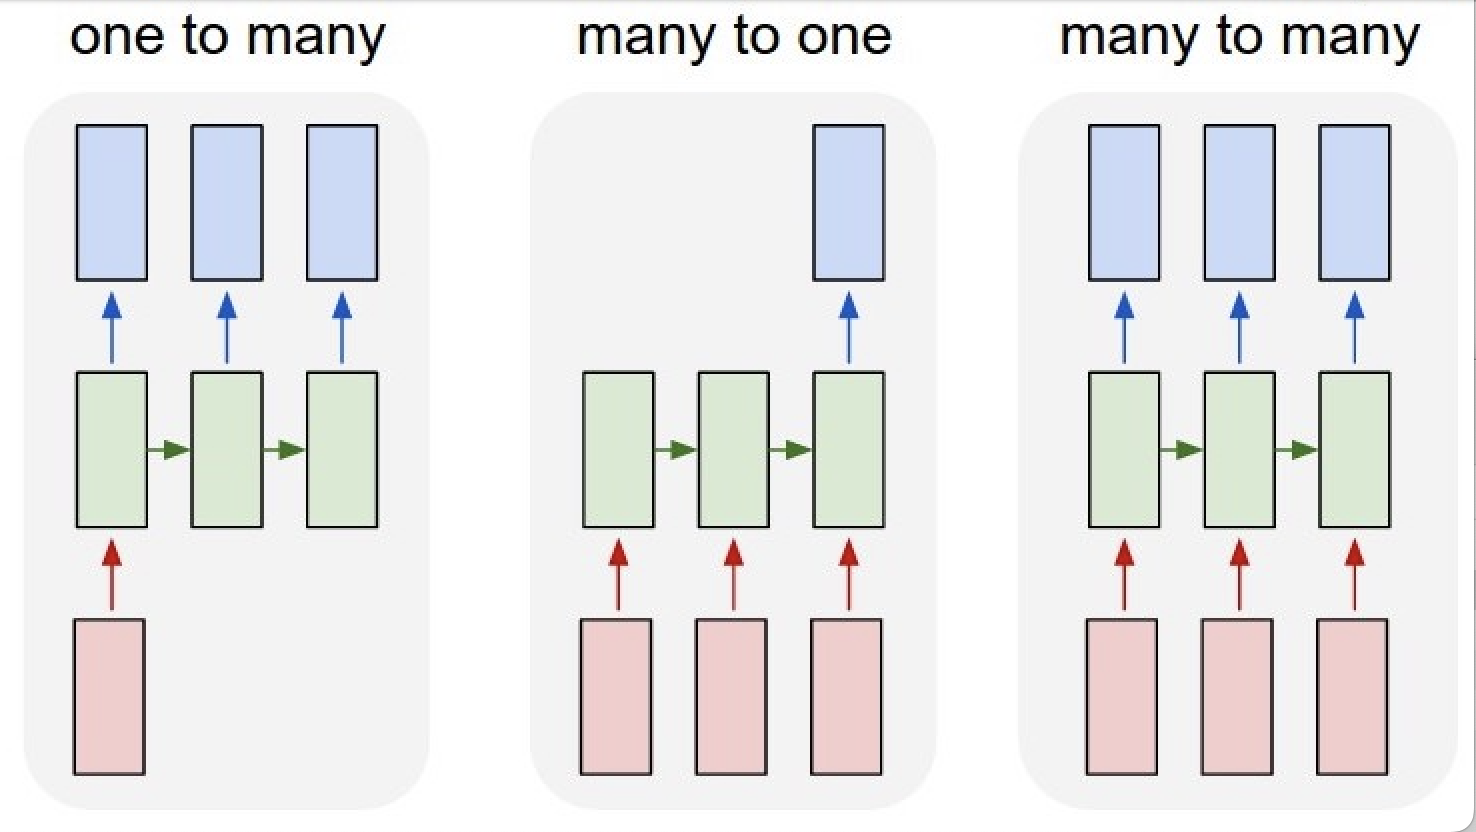
\includegraphics[scale=.4]{images/karpathy_rnn.png}}
\caption[Adapted from Karpathy, 2015 \cite{karpathy2015unreasonable}.]{Different types of sequence learning possible with backprop through time.}
\label{rnn_schema}
\end{figure}
% TODO: Update caption

These ideas have links to dynamical systems theory (chapter \extref{ch_dst}). In the single input vector (one to many) case we are training the network to produce an orbit in the output space relative to an initial condition triggered by the input. Variations on this architecture and this method can be used to train a network to produce a whole phase portrait. In fact, there are theorems which show that recurrent networks can in principle produce any trajectory of any dynamical system \cite{funahashi1993approximation}.\footnote{Even more generally a recurrent network can reproduce any Turing Machine, and hence \emph{any computational system}. They are ``Turing Complete''; see \cite{haykin1998neural} section 15.5; also see \url{http://binds.cs.umass.edu/papers/1995_Siegelmann_Science.pdf}. These results are comparable to the universal approximation theorem for feed-forward networks noted in chapter \extref{ch_lms_backprop}} 
% Abstractly, that is what is happening with the weird examples in the next section. We train it on some sequences in a linguistic space, etc.

There are clearly many applications here. Again, many are in the domain of natural language: chat bots, sentiment analysis, text summarization, speech recognition, machine translations. But there are other applications: time series forecasting, video classification, video captioning, music generation, music recognition,  video acton recognition (identifying objects in a video or determining what is being done), etc (for each case, ask which category it fits best in).  As we will see, the technology is rapidly changing in this area, since it has so many applications, but cognitive science and neuroscience are paying close attention, and this material continues to be highly relevant to understanding the human mind and brain.

\section{Simple Recurrent Networks}

To begin to understand how these networks work, and how they were used in cognitive science, we can consider an old class of model, the \glossary{simple recurrent network} or SRN, which was developed by Jeff Elman \cite{elman1990finding}, a member the original PDP research group  (in fact, they are also sometimes called ``Elman networks''). SRNs are important because (1) they show what the basic approach to training recurrent networks is, and (2) because they were used by connectionists to demonstrate how grammars could be learned by a network. 
% Elman's paper containers the longer history of the method. Jordan had a similar idea but the context layer copied the outputs, not hidden units.

The structure of an SRN is shown in Fig. \ref{SRN_Structure}. It is basically a regular 3-layer feed-forward network trained using backpropagation, with some special machinery for processing temporal context.The special feature is the ``last hidden state'' portion of the input layer, which is always set to the hidden layer activation vector of last time step (in the first time step it is usually just set to the  zero vector).\footnote{ As McClelland says,``The beauty of the SRN is its simplicity. In fact, it is really just a three-layer, feed-forward back propagation network. The only proviso is that one of the two parts of the input to the network is the pattern of activation over the network's own hidden units at the previous time step'' \url{ https://web.stanford.edu/group/pdplab/pdphandbook/handbookch8.html}.} It is a ``copy-back'' of the hidden  layer. Otherwise it is like another part of the input layer, fully connected to the hidden layer. Thus at any time the full input to the network is the current input, \emph{plus some temporal context}. It's a bit like  someone saying ``Good times!''. At the moment you hear them say ``times!'' you have some memory of them having just said ``Good''. You  hear ``times!'' in the context of ``Good''. This allows you to distinguish ``good times'' from ``bad times'' from ``crazy times'', etc.\footnote{This idea occurs in philosophy in the work of Edmund Husserl and others who claimed that human experience essentially involves ``time consciousness'', which in turn includes an awareness of what has just-passed and what is about to come (and note that SRNs are usually trained to predict one step in the future). See \url{https://plato.stanford.edu/entries/consciousness-temporal/}.}$^,$\footnote{But note it's not the past input that is remembered, it's the past  hidden state. That hidden state is influenced by the past  input, \emph{and} earlier hidden states. Thus there is a recursive relationship here that allows the temporal influence to extend arbitrarily far back in the past, though the influence is strongest in the recent past.}

\begin{figure}[h]
\centering
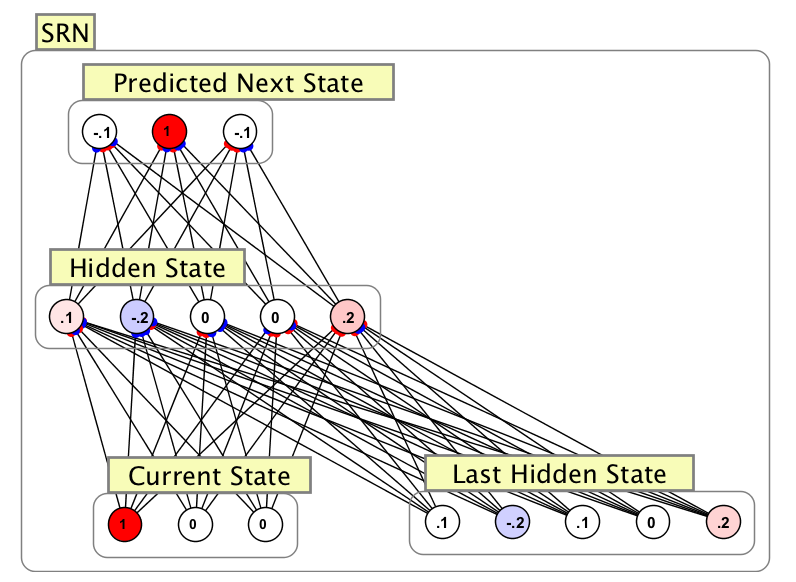
\includegraphics[scale=.6]{./images/srn.png}
\caption[Simbrain screenshot.]{A simple recurrent network.}
\label{SRN_Structure}
\end{figure}

SRNs are also trained in a special way. They use a training dataset, like the ones discussed in chapter \extref{ch_supervised}, and shown below. But unlike a normal training dataset, the rows of an SRN's dataset must be presented in a specific temporal order. As each input vector is presented to the network, the output is computed based on that input vector, \emph{and} on the hidden layer vector from the last time step. Then backprop is used in the usual way to update all the weights of  the network. Table \ref{userProvidedSRN} shows an example of a training set for a recurrent network. To emphasize the importance of temporal order, a column for time has been added.
 
 \begin{table}
\begin{center}
\begin{tabular}{| c || c | c | c || c | c | c | }
\cline{1-7}
\multicolumn{1}{| c || }{time} 
& \multicolumn{3}{| c || }{inputs} 
 & \multicolumn{3}{c |}{targets} \\
\hline
1 &  1 & 0 & 0 & 0 & 1 & 0   \\
\hline
2 & 0 & 1 & 0 & 0 & 0 & 1 \\
\hline
3 & 0 & 0 & 1 & 0 & 1 & 0  \\
 \hline
 4 & 0& 1 & 0 & 1 & 0 & 0   \\
\hline
 5 & 1 & 0 & 0 & 0 & 1 & 0  \\
\hline
\end{tabular}
\end{center}
\caption{The user provided training set for an SRN. We say what outputs we want to occur, in what order, given a time-ordered sequence of inputs. Note there is a puzzle: the state $(0,1,0)$ occurs twice, with two different outputs, and thus seems to pose a problem for training.}
\label{userProvidedSRN}
\end{table}

% TODO: Link to transformers, move all of it to nlp?
% Shift registers.
 The dataset trains an SRN on a one-step prediction problem, which is often what SRNs are used for. In machine learning contexts this type of training is also common; there they are referred to as ``auto-regression'' tasks.  The network learns to predict the next item in a sequence based on what items have occurred before. A nice thing about this kind of task is that there is no need for ``labeled data.'' Any string of words or tokens is enough to train a network, since the target at any time is just the next item in a sequence. 
 
In the toy example being considered here, the network is being trained on a ``bouncing one'' pattern. For example, if we enter $(1,0,0)$, the SRN should predict that $(0,1,0)$  comes next. But notice that the vector $(0,1,0)$ is ambiguous. It will predict \emph{different} outputs depending on when we present it. It predicts  $(1,0,0)$ after  $(0,0,1)$, but  $(0,0,1)$ after  $(1,0,0)$. How can the network do this? The answer is: by using the context  layer. The last hidden state after seeing $(1,0,0)$ is different then it is after seeing $(0,0,1)$. This allows the network to differentiate the same input, $(0,1,0)$, in different temporal contexts. 
 
 In fact, behind the scenes, what is happening is that the network uses regular backprop, but with a special training set. The real training set, ``under the hood'', is shown in table \ref{underHoodSRN}.  The network learns to associate inputs with outputs, \emph{in the context of specific hidden layer states}. Notice that the last hidden unit state at time 2 is different from the last hidden unit state at time 4. This allows the network to solve the problem.
% This can be done in Simbrain, but it requires care (which is perhaps instructive). The initial state must be initialized the same way, and the exact sequence of inputs must be used, so that last hidden states are preserved.

\begin{table}
\begin{center}
\begin{tabular}{| c || c | c | c || c | c | c | c | c  || c | c | c | }
\cline{1-12}
\multicolumn{1}{| c || }{time} 
& \multicolumn{3}{| c || }{inputs} 
& \multicolumn{5}{| c || }{last hidden} 
 & \multicolumn{3}{c |}{targets} \\
\hline
1 & 1 & 0 & 0 & .5 & .5 & .5 & .5 & .5 & 0 & 1 & 0   \\
\hline
2 & 0 & 1 & 0 & 0.9 & 0.9 & 0.9 & 0.2 & 0.9 & 0 & 0 & 1 \\
\hline
3 & 0 & 0 & 1 & 0.4 & 0.8 & 0.8 & 0.9 & -0.2 & 0 & 1 & 0  \\
 \hline
 4 & 0& 1 & 0 & 0.9 & 0.9 & 0.9 & -0.2 & 0.9 & 1 & 0 & 0   \\
\hline
 5 & 1 & 0 & 0 & 0.9 & 0.3 & 0.3 & 0.9 & -0.5 & 0 & 1 & 0  \\
\hline
\end{tabular}
\end{center}
\caption{The actual training set used ``under the hood'' by the SRN.  The inputs are external inputs together with the last hidden state of the network, which reflects recurrent dynamic processing. This allows the network to disambiguate the $(0,1,0)$, which is different in its two temporal contexts, where the last hidden state is different.}
\label{underHoodSRN}
\end{table}
 
 We can train these networks on arbitrarily long sequences, like all the sentences in a document, or all the images in a movie, or all the sounds in a musical piece, assuming of course that the sentences, images, or sounds have been converted into vectors (see the discussion of feature encoding in chapter \extref{ch_data_science}). As we will see, the hidden layer can then be  analyzed for the patterns it discovers and the sequences of patterns it goes through in time. In psychology, SRN's have been especially useful at studying the development of linguistic categories in networks that learn to predict the next sound in a speech stream, or the next word in a passage of text.

\section{Backpropagation Through Time}

% BPTT was used in cog-sci way back. Add some discussion of earlier uses. 
% The update is like this: We first update the time 1 ff net, then update the time 2 ff net so it gets the time 2 input and the hidden activations from the time 1 net, etc. So we can't really jus update it in one go like a normal ff network, we actually have to update from left to right as it were. 



A more general framework for training recurrent networks (which can be thought of as generalizing the SRN to include arbitrarily many time steps in the past) is by using ``backpropagation through time'' \cite{werbos1990bptt}.\footnote{There are other methods of training recurrent networks, eg. real time recurrent learning \cite{williams1989learning}, and ``dynamic reconstruction'' (Haykin, 14.13) \cite{haykin1998neural}.} As with the SRN, we start with a simple three-layer feed-forward network, but instead of a ``copy back''  layer, we use a recurrent layer of weights from the hidden layer back to itself. Like the SRN, we have a training dataset that involves time ordered input-target pairs. In order to train the network, we ``unroll'' the network so that all the inputs can be put in the network at the same time. It's as if you take the original network, copy and paste it a bunch of times (once for each row of your training set), and then replace the recurrent weights from the hidden layer back to itself with lateral weights \emph{between} the copy-pasted hidden layers (see figure \ref{bptt}). 

% A bit easier to understand when shown "diagonally", maybe with time indicators to show how the inputs are added and computed.
\begin{figure}[h]
\centering
\frame{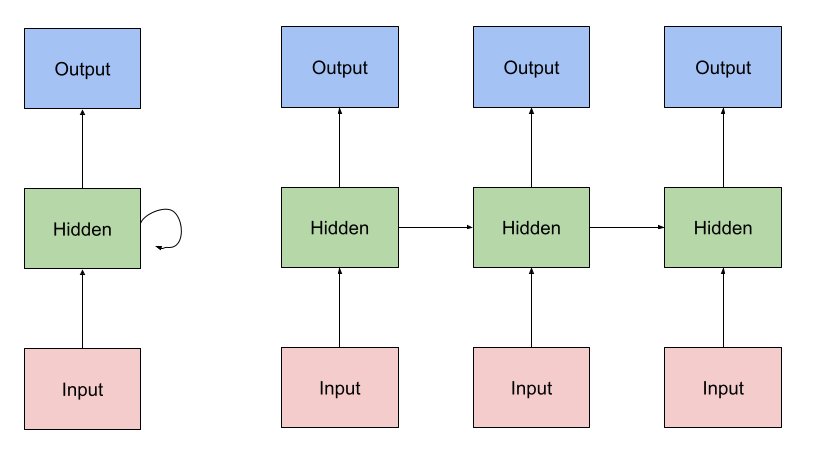
\includegraphics[width=0.5\textwidth]{images/BPTT.png}}
\caption[Jeff Yoshimi.]{Schematic of backprop through time. The actual network that we are training is on the left: a feed-forward network with a recurrent weight layer in the middle. The unrolled network is on the right. This network can learn a sequence of three input-target pairs. We train the unrolled network to produce target values in response to current inputs \emph{and} to previous hidden layer states. When training is done, the changes to the weight matrices (the arrows) are added together and so we have ``rolled the network back up'' to the network on the left.}
\label{bptt}
\end{figure}

% TODO: Below does not make sense. That should be each "column" of the single unrolled network or something.

% This needs to be double checked. Also the "re-rolling'' is not just adding, it's also averaging. Some of the footnote material can be improved and promoted.
Each of the unrolled networks is then responsible for a specific moment in time. To train the network, we put together all the inputs in the dataset into one long input, one for each of the unrolled networks. Then we train the whole unrolled network to produce the corresponding sequence of outputs.\footnote{This involves exposing the network to each of the inputs in a sequence from left to right, so that hidden layer activations are updated in a specified order. This hidden layer activations provide contextual disambiguation in the same way the copy-back later does in a SRN. The resulting sequence of outputs is compared to the target output sequence, producing an error, which is backpropogated.} But you are not just training the usual weights from input-to-hidden layer and from hidden-to-output layer. You are also training the hidden-to-hidden weights in the middle, that laterally connect the hidden layers  of the unrolled network to each other. Note that the unrolled network is really just a feed-forward network, with some extra lateral weights. So this is ultimately a trick to use feed-forward methods on a recurrent network! When we are done training this big unrolled network, we add up all the input-to-hidden, hidden-to-hidden, and hidden-to-output weight matrices, which is like collapsing the unrolled network back to down the original network, the one on the left side of figure \ref{bptt}. If we present the network with a sequence of input vectors from the training set, in sequence, it should produce the same sequence of target vectors. And, it should generalize, producing similar sequences of outputs to those in the target set, given a similar sequence of inputs. 

%The network on the left side of figure \ref{bptt} is what the neural network really looks like, the network we will eventually use to do things. Each colored box is a layer of a network, a layer that can have 1 or 2, or maybe 100 or 1000 nodes in it. So this is a kind of zoomed-out view of a 3 layer feed-forward network, where all we see are node layers, not the nodes themselves. The arrows correspond to weight matrices, or weight layers. 

%The unrolled network is on the right. It involves a copy-paste of the same network three times, with the recurrent weights presented as the left-to-right arrows in the middle. Time flows from left to right and each ``column'' (each 2 or 3 layer feed-forward network)  represents one time step. It is being trained on a sequence of three input-target pairs. We present the first input to the first network, compute the output at time 1, then present the second input to the second layer \emph{and also add the activations from the hidden layer at the previous time step}.\footnote{Again, this is a lot like an SRN, since in both cases the hidden layer is receiving a ``visible'' input as well as the hidden layer's previous activation as a second invisible input.}  The output at time 2 then reflects both past inputs: it knows about context. We keep doing this until we reach the end. We have three time steps here, but we can use as many as we have computer memory to handle. Then we train the whole thing with backpropagation. But note, the various arrows on the right side correspond to a bunch of copies of the same weight matrices. So when a pass of training is done, they all get added back together and what we end up with is just the network on the left.

\section{Recurrent Networks and Language Generation}\label{languageModelsRecurrent}

% Word embedding link
Once various technical issues with training recurrent networks were resolved as part of the deep learning revolution, people started using them to do truly amazing things, in particular, build models of language that could generate text. This was a precursor to large language models, and was at the time quite amazing.

In a now-classic blog post, Andrej Karpathy describes some of these applications.\footnote{\url{http://karpathy.github.io/2015/05/21/rnn-effectiveness/}. Note that Karpathy makes use of LSTMs; see note \ref{lstm}.}  For example, he trained a neural network on a bunch of Shakespeare\footnote{The data is here: \url{http://cs.stanford.edu/people/karpathy/char-rnn/shakespear.txt}.}  (with words coded as vectors, of course) and then ran the RNN, which produced it's own version of Shakespeare \cite{karpathy2015unreasonable}. Here is a sample:
% These are called language models. More specifically character level models because they predict the next character in a sequence.

\begin{quotation}
\hspace{5em} \\
VIOLA: \\ \\
\emph{Why, Salisbury must find his flesh and thought \\
That which I am not aps, not a man and in fire, \\
To show the reining of the raven and the wars \\
To grace my hand reproach within, and not a fair are hand}
\end{quotation}

In another example Karpathy trained a network to speak like Tolstoy using an English Translation of \emph{War and Peace}. Remember, these are just networks' trained using variations on backprop.  So he would train the network to produce sequences of statements that were similar to sequences of statements in Tolstoy. As the network learns using gradient descent, the outputs seem more and more like Tolstoy. Recall how we could track Nettalk learning to speak at different stages of training, like a creepy baby (section \extref{ch_representations}). Here we can do the same thing with the network, observing get better and better at speaking in the voice of Tolstoy. Here is some network output after iteration 100:

% https://tex.stackexchange.com/questions/2396/how-can-i-change-the-indentation-in-quote-and-quotation-environments-and-command
\newenvironment{myquote}
  {\list{}{\leftmargin=0.3in\rightmargin=0.3in}\item[]}
  {\endlist}
\begin{myquote}
tyntd-iafhatawiaoihrdemot  lytdws  e ,tfti, astai f ogoh eoase rrranbyne 'nhthnee e 
plia tklrgd t o idoe ns,smtt   h ne etie h,hregtrs nigtike,aoaenns ln
\end{myquote}
The network doesn't even really have the concept of a word yet. By iteration 700 it has words, kind of:
\begin{myquote}
Aftair fall unsuch that the hall for Prince Velzonski's that me of
her hearly, and behs to so arwage fiving were to it beloge, pavu say falling misfort 
how, and Gogition is so overelical and ofter.
\end{myquote}
Finally, after a few thousand iterations, it's beginning to sound like a Russian novel:
\begin{myquote}
``Why do what that day,'' replied Natasha, and wishing to himself the fact the
princess, Princess Mary was easier, fed in had oftened him. Pierre asking his soul came to the packs and drove up his father-in-law women.
\end{myquote}

Karpathy got these supervised recurrent networks to do other cool things:  for example, he generated a fake wikipedia page, fake source code, and a fake math paper \cite{karpathy2015unreasonable}. A fragment from the artificially generated mathematics paper is shown in Fig. \ref{fakeMath}. These techniques have even been used to generate a fake script for a movie, which was then actually produced!\footnote{The move is called ``Sunspring'', and can be viewed here: \url{https://www.youtube.com/watch?v=LY7x2Ihqjmc}. The opening shows a list of all the other movie scripts that were used to train the network to produce its script \cite{newitz2016movie}}

\begin{figure}[h]
\centering
\frame{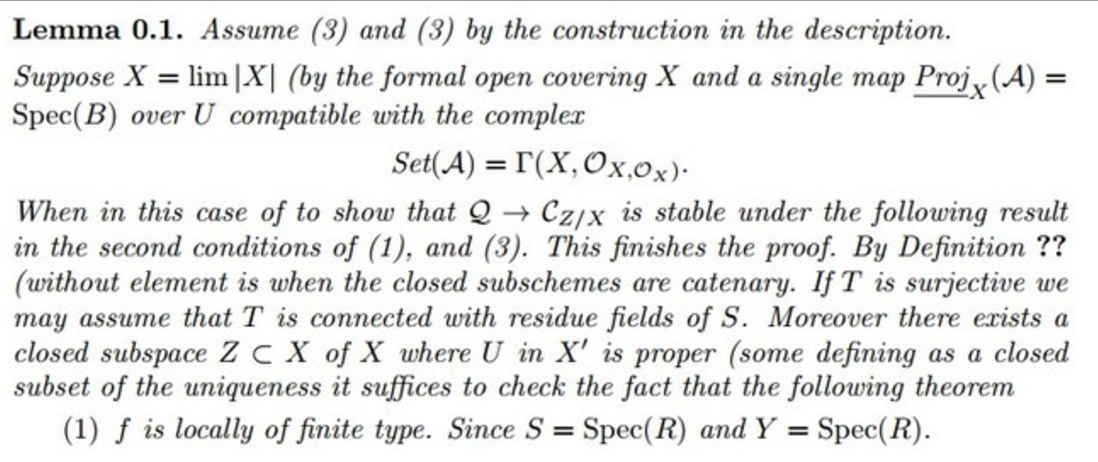
\includegraphics[width=0.7\textwidth]{images/recurrentMath.png}}
\caption[From Karpathy, 2015 \cite{karpathy2015unreasonable}.]{Fragment of ``fake math'' generated by a recurrent network trained on real math.}
\label{fakeMath}
\end{figure}

\section{Limitations of Supervised Recurrent Networks}\label{supervisedRecurrentLimitations}

Karpathy's blog post was written in 2015. In 2020, GPT was released, and in 2022, ChatGPT was publicly released, and thus began the next era in the history of neural networks, which we are currently living in. See chapter \ref{ch_transformers}. In a way, those advances grew out of efforts to overcome limitations of supervised recurrent networks like the one's we've described.

We've seen that recurrent connections can provide a network with context information (for example with the copy-back layer of a SRN). What the network sees at time $t$ is an external input and some trace of what happened in the past.  Input plus context is enough for the network to learn to produce meaningful temporal sequences. Transformer networks improve on this basic idea. The main problem they run into is that they favor recent context over earlier context.  But oftentimes it is important to be more sensitive to information much earlier in a sequence than more recent information, and as a result recurrent networks have a hard time capturing larger temporal structures,  like the plot of a story or the overall theme of a musical performance. 

There are also technical problems, like the the problem of vanishing gradients: as error is backpropagated through the weights of a network (section \extref{backprop}), the amount weights are changed further back in time gets smaller and smaller. Another problem is that this type of network does not lend itself to parallel computing hardware like GPUs on fancy graphics cards. This can be dealt with using some tricks, like truncating how far back the ``window'' of backprop goes (``truncated'' backprop through time), but this only takes us so far.
%% In fact they bear some resemblance to those who suffer from antero-grade amnesia (cf. the piano performances of someone like Clive Wearing, who can create beautiful music but can no longer produce long pieces). Better develop this point with citations. 

One approach to this problem is to use nodes with more complex activations functions (see chapter \extref{ch_act_functions}).\footnote{Two such functions are ``long-short-term memories'' (LSTMs)  \cite{schmidhuber1997long, olah2015understanding} and ``gated recurrent units'' (GRUs). See \url{http://colah.github.io/posts/2015-08-Understanding-LSTMs.} These functions---which are like compound activation functions containing several others as parts---allow activations to be gated or turned off altogether. When placed in a recurrent network trained using gradient descent, they can learn to pass information far along a temporal sequence, ``jumping'' over intermediate nodes, in a way that avoids the problem of vanishing gradients.\label{lstm}} However, these approaches have not been discussed much in connection with cognitive science, and are being supplanted by other techniques, so we pass over them for now. 
% GPT: For certain applications like speech recognition, time series forecasting, and tasks where the data has strong temporal dependencies, LSTMs can still perform competitively. While Transformers are strong for many NLP tasks, LSTMs may be preferable in some sequential domains where modeling step-by-step temporal dependencies is more straightforward.  [Also easier to implement, work on smaller data, just straight-forward for small datasets.]


%TODO
The answer was to drop recurrent networks, in a sense, and move back to feed-forward.

\section{Connectionist Applications}\label{internalRepsRecurrent}

Having reviewed the latest and greatest in supervised recurrent networks, let us return to earlier and simpler models, to examine their relevance to cognitive science.

% Add more about Elman's reps. The different cases, in particular breaking up the speech stream. Mention Simbrain sim.  And see book todos for important notes on how this works.

In Chapter \extref{ch_supervised} we saw that multilayer networks trained by supervised learning methods (e.g. backprop) can develop psychologically interesting internal representations that involve a re-mapping of inputs in a hidden layer. Thus backprop is relevant to psychology even if it is not neurally realistic. Similar work has been done with supervised recurrent networks. 

In a famous paper, Jeff Elman trained a simple recurrent network like the one in figure \ref{SRN_Structure} to predict the next words in a sentence.\footnote{\url{http://psych.colorado.edu/~kimlab/Elman1990.pdf}.}  The input data used to train the network consisted of thousands of sentences generated using a simple ``caveman'' grammar. Some sample sentences generated by this grammar are shown in Fig. \ref{elman_sentences}. The network predicts the next word in  a sentence at any time. For example, it predicts that the word ``cat'' will be followed by ``chase'' or ``eat''. With training, error can be reduced, but it never goes to zero, because a given word can be followed by more than one other word. But some words are more likely than others to follow one another, and so the predictions match these patterns. It also learns some general rules, like expecting verbs after nouns \cite{elman1990finding}.\footnote{Simbrain simulations that partially replicate the results of these papers can be accessed in the script menu as \texttt{elmanPhonemes.bsh} and \texttt{elmanSentences.bsh}.}

\begin{figure}[h]
\centering
\frame{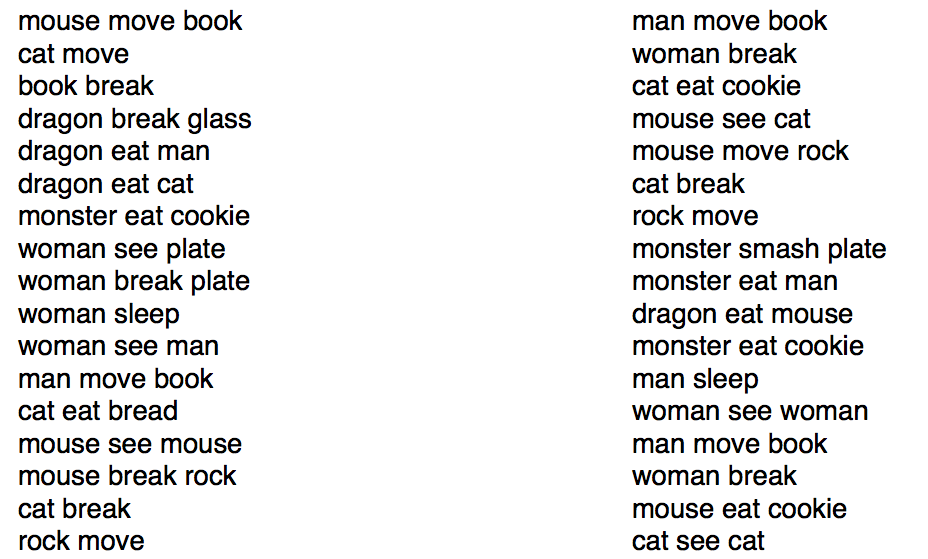
\includegraphics[width=0.65\textwidth]{images/elman_sentences.png}}
\caption[Generated by Jeff Yoshimi based on \cite{elman1990finding}.]{Some of the sentences used to train the word prediction network.}
\label{elman_sentences}
\end{figure}

The striking thing about this network was that it learned a set of grammatical categories in its hidden layer, \emph{without being told anything about grammar}. The internal representations the network learned corresponded to grammatical categories like noun and verb, as well as semantic categories like animal, human, food, and breakable. None of these categories were directly programmed in to the network: it simply learned these categories in the process of solving the input-output task it was given (compare the way Nettalk learned phonological categories when learning to read aloud, or the way deep networks develop realistic edge detectors and other feature detectors when trained to recognize objects). 

Figure \ref{srn_words} shows a schematic reconstruction of the structure of the SRN's hidden unit space.\footnote{The picture this is based on was generated by exposing the network to each word in the context of many sentences (\eg ``eat'', ``cat''), and then taking the average hidden unit activation across these exposures. The resulting vectors are like the centers of clusters in the hidden unit space.} Points correspond to vectors in the hidden unit space. Distances between points are meaningful: points closer to each other in the diagram correspond to hidden unit vectors that are closer to each other in the hidden unit space. Notice that the internal representations form in to a kind of hierarchical structure, that mirrors the structure of English grammar and also some features of English semantics. Nouns are broadly separate from verbs. Within nouns we have animate vs. inanimate nouns. 

The network was used to argue against the prevailing view in psycholinguistics, associated with Noam Chomsky,  that  grammars are innate, rather than learned. The rules of grammar were not given to the network. They were learned by the network when it was trained to predict the next word in grammatical sentences \cite{elman1990finding}. The grammar was in the environment--it was implicit in the sentences of the training dataset--and then learned by the network.
% Written quickly; carefully revise and add citations before publication.

\begin{figure}[h]
\centering
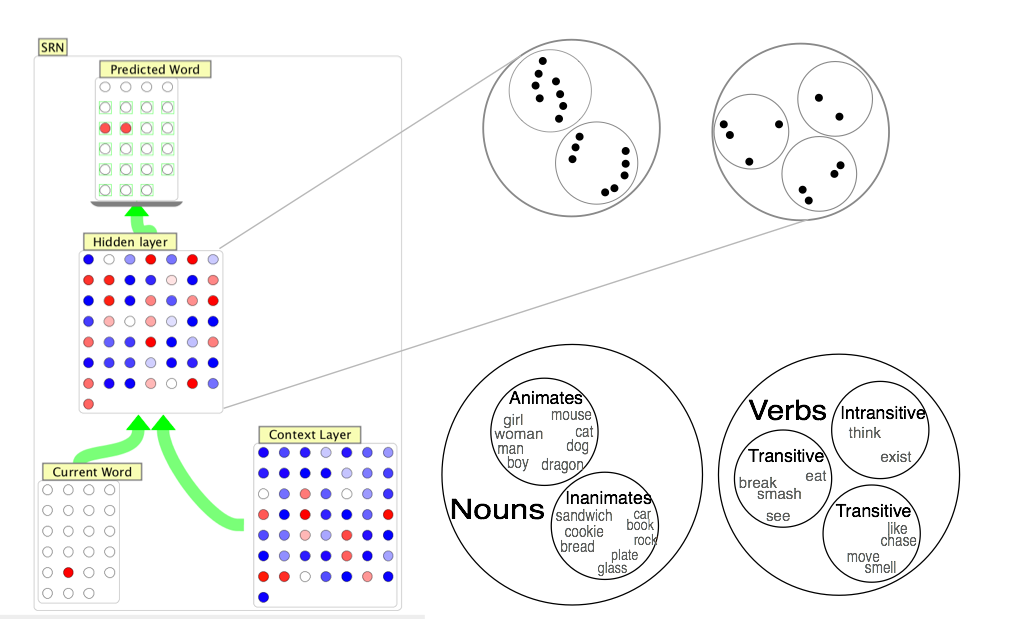
\includegraphics[width=0.7\textwidth]{images/elmanCategories.png}
\caption[Pamela Payne.]{The SRN used in the word prediction task. The output layer predicts the next word (coded as a binary vector) in a sentence. It is currently undecided between which of two words might come next. The right top panel shows (schematically, this is not a projection of actual data) what points in the hidden unit space corresponding to different words. The right bottom panel shows how these points cluster in to grammatical and semantic categories.}
\label{srn_words}
\end{figure}

This is a good example of connectionism. Elman used backprop to show neurally plausible processes could capture psycho-linguistic phenomena, without claiming to show exactly what was happening in the brain.

A final, more recent example, shows that these ideas persist, even among those who are not concerned with cognitive science or psychology. Karpathy's amazing recurrent neural networks, which learned to generate fake math texts, encyclopedia pages, and source code, were also analyzed for internal representations. The results were fascinating. Some nodes only turned on when the network was producing text inside of quotations. Other nodes only turned on at the beginnings and ends of lines. Other nodes kept track of opening and closing brackets or parentheses \cite{karpathy2015visualizing}. 

This is by no means a settled area.  As discussed in section \extref{llm_cogsci}, linguistic processing using transformers has become a whole sub-field of computational linguistics, known as BERTology. The question of what kind of meaningful representations develop in other language models trained using transformers, such as GPT-3, is a natural direction for further research. To take just one example, in the paper referenced above  \cite{mcclelland2020placing}, it is argued that the human cognitive system uses some variant on a transformer model, what they call ``query based attention'' or QBA. They note: ``Some attention-based models (28) proceed sequentially, predicting each word using QBA over prior context, while BERT operates in parallel, using mutual QBA simultaneously on all of the words in an input text block. Humans appear to exploit past context and a limited window of subsequent context (29), suggesting a hybrid strategy.'' They argue that this context is not just linguistic, but encompasses a whole situation we are in, and that we use this situational context---what we see, hear, are doing etc.---to disambiguate words in context. 
% Refer back to the discussion of connectionism as system identification.
